%**************************************************************************
%                                        PLANTILLA PARA REPORTE DE SECO
%**************************************************************************
\documentclass[final]{beamer}

% ====================
% Paquetes
% ====================

\usepackage[T1]{fontenc}
\usepackage{lmodern}
\usepackage[size=custom,width=120,height=86,scale=1.0]{beamerposter}
\usetheme{gemini}
\usecolortheme{uci}  % or uci_dark
\usepackage{graphicx}
\usepackage{booktabs}
\usepackage{tikz}
\usepackage{pgfplots}
\pgfplotsset{compat=1.14}
\usepackage{anyfontsize}

% ====================
% Lengths
% ====================

% If you have N columns, choose \sepwidth and \colwidth such that
% (N+1)*\sepwidth + N*\colwidth = \paperwidth
\newlength{\sepwidth}
\newlength{\colwidth}
\setlength{\sepwidth}{0.025\paperwidth}
\setlength{\colwidth}{0.3\paperwidth}

\newcommand{\separatorcolumn}{\begin{column}{\sepwidth}\end{column}}

% ====================
% Titulo
% ====================

\title{Boletin del Sector Café en Honduas}

\author{Autor \inst{1} \and Autor \inst{2} \and Autor \inst{3}}

\institute[shortinst]{\inst{1} Grupo Financiero Ficohsa \samelineand \inst{2} Riesgos}

% ====================
% Footer (optional)
% ====================

\footercontent{
  \href{https://www.ficohsa.hn/}{https://www.ficohsa.hn/} \hfill
  Gestión Integral de Riesgos \hfill
  \href{Ciencia de datos}{Ciencia de Datos}}
% (can be left out to remove footer)

% ====================
% Body
% ====================

\begin{document}

% Refer to https://github.com/k4rtik/uchicago-poster
% logo: https://www.cam.ac.uk/brand-resources/about-the-logo/logo-downloads
\addtobeamertemplate{headline}{}
{
    \begin{tikzpicture}[remember picture,overlay]
      \node [anchor=north west, inner sep=3cm] at ([xshift=0.0cm,yshift=0.5cm]current page.north west)
      {
\includegraphics[height=3.5cm]{logos/logo.png}};
      % {\includegraphics[height=3.5cm]{logos/university-of-california-irvine-uci-vector-logo-wordmark-white.eps}};
    \end{tikzpicture}
}

\begin{frame}[t]
\begin{columns}[t]
\separatorcolumn

\begin{column}{\colwidth}

%====================================================
%                                                        BLOQUE 1
%====================================================
  \begin{block}{Contexto general}

    El \textbf{sector cafetalero hondureño} continúa siendo uno de los pilares de la economía nacional, representando aproximadamente el 5\% \textbf{del PIB total} y cerca del 20\% \textbf{del PIB agrícola}. Además, genera más de \textbf{120 mil empleos directos} y constituye la \textbf{principal fuente de divisas del sector agroexportador.}\\[0.4cm]

   Sin embargo, el entorno actual presenta \textbf{retos significativos}. Tras alcanzar un récord histórico de \textbf{7.29 millones de sacos exportados en la cosecha de 2016-2017}, el volumen cayo a \textbf{4.68 millones de sacos en la cosecha 2023-2024}, lo que equivale a una \textbf{reducción del 36\%}. Esta contracción responde a una combinación de factores como la \textbf{volatilidad en los precios internacionales, condiciones climáticas adversas} y \textbf{aumentos en los costos de producción y transporte}.  
   
   \begin{center}
    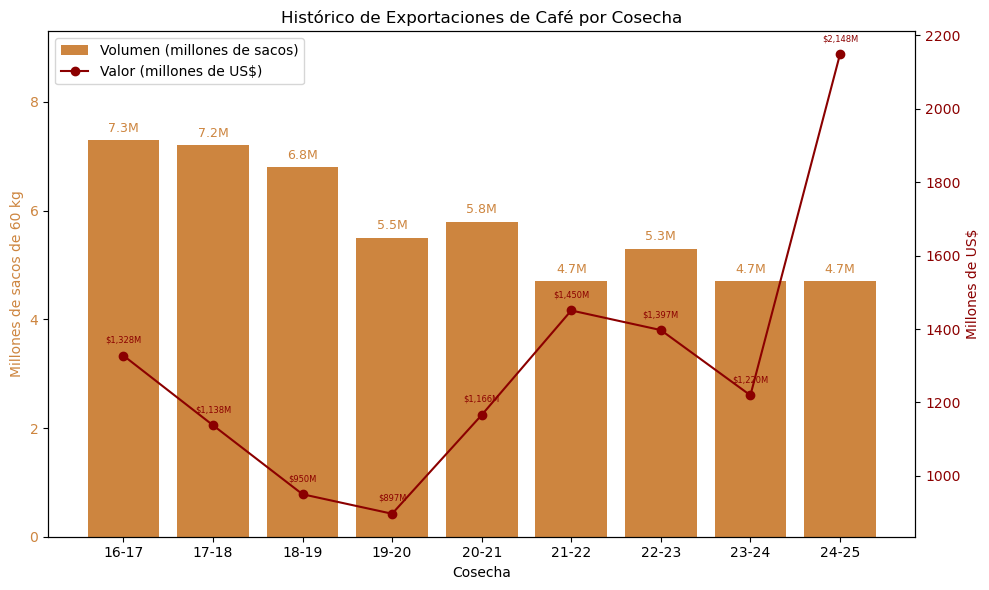
\includegraphics[scale=0.55]{fig1.jpg}
   \end{center}

Al mismo tiempo, las \textbf{expectativas de precios futuros} muestran signos mixtos: mientras los contratos en la bolsa de Nueva York (ICE Coffe C) se mantienen por encima del promedio histórico, los \textbf{margenes de rentabilidad del productor} se han visto presionados por la inflación y la apreciación del dólar.\\[0.4cm]

En este boletín, elaborado por el área de \textbf{Gestión Integral de Riesgos} y \textbf{Ciencia de Datos de Grupo Financiero Ficohsa}, se analiza la \textbf{coyuntura actual del sector café}, sus principales \textbf{riesgos microfinancieros} y la \textbf{calificación del sector según el modelo IRSS (Índice de Riesgos Sectorial Sistématico)}, con el fin de apoyar la \textbf{toma de decisiones estratégicas de crédito y apetito de riesgo} institucional.

  \end{block}
%====================================================
%                                                        BLOQUE 2
%====================================================
  \begin{block}{Desempeño reciente del sector cafetalero}

De acuerdo con datos de ADECAFEH e IHCAFE, durante la cosecha 2023-2024 las exportaciones de café hondureño se estabilizaron en torno a \textbf{4.68 millones de sacos de 60kg}, cifra que confirma la \textbf{moderación en la producción} tras varios años de ajustes estructurales en el sector. Aunque el volumen continúa por debajo del máximo histórico alcanzado en 2016-2017, el \textbf{valor exportado mostró una recuperación parcial} gracias a mejores precios internacionales y a una \textbf{mayor participación de cafés diferenciados (orgánico, RFA, FLO, entre otros).}\\[1cm]

El repunte observado en el valor de exportación responde principalmente a \textbf{factores de mercado externos}, más que aun aumento en la productividad local, lo cual mantiene al sector \textbf{expuesto a la volatilidad de precios} y a las \textbf{condiciones climáticas} que afectan la oferta mundial. \\[1cm]

En este contexto, el \textbf{IRSS}, modelo desarrollado por el área Gestión Integral de Riesgos y Ciencia de Datos permite \textbf{cuantificar el nivel de vulnerabilidad y estabilidad relativa} del sector frente a factores macroeconómicos, financieros y productivos. \\[1cm]

Según la estimación más reciente, el IRSS del sector café se ubica en XXXXXX (nivel bajo), lo que refleja una exposición baja al riesgo sistémico, sustentada en precios favorables pero con alta sensibilidad a choques externos.

   

  \end{block}
%====================================================
%                                                        BLOQUE 3
%====================================================
  \begin{block}{Factores macroeconómicos y exposición crediticia}

{Según el IRSS, el comportamiento de ciertos indicadores o variables condiciona directamente la capacidad de pago del sector cafetalero y el nivel de riesgo que asume el banco al otorgar créditos agrícolas. Estas variables son: }
{\small
\begin{itemize}
\item \textbf{VENTA\_ENERGIA:} ventas de energia de la ENEE.
\item \textbf{SPI3\_ELPA:} índice de precipitaciones acumulado de 3 meses en el Paraíso.
\item \textbf{SPI3\_AGA:} índice de precipitaciones acumulado de 3 meses en Agalta.
\item \textbf{WTI14:} Precio global actual del petróleo.
\item \textbf{IPI\_USA:} índice de producción industrial USA.
\item \textbf{REAL\_EX\_BR:} Tipo de cambio real del real brasileño.
\item \textbf{X\_CAFE\_BR:} Exportaciones de café de Brasil.
\item \textbf{PCA1\_xcafé:} Componente principal o índice sintético de las exportaciones de café.
\end{itemize}
}
{ Estas variables permiten capturar los efectos combinados de la demanda energética, el clima, la producción internacional y las condiciones cambiarias sobre el desempeño del sector cafetalero. En conjunto, explican una proporción significativa de la variabilidad del riesgo crediticio observado en el portafolio agrícola de Ficohsa.}
  \end{block}

\end{column}

\separatorcolumn

\begin{column}{\colwidth}
%====================================================
%                                                        BLOQUE 4
%====================================================
  \begin{block}{Resultados del modelo IRSS y análisis de riesgo}
   
   \begin{center}
    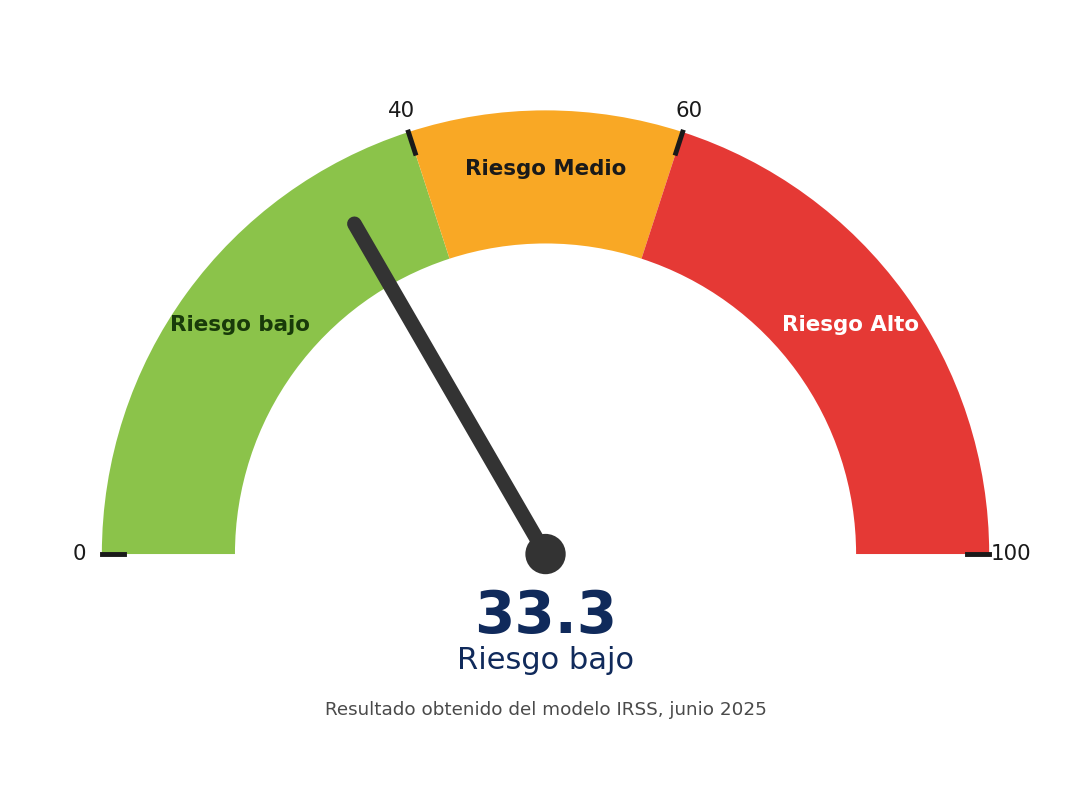
\includegraphics[scale=1.2]{fig2.png}
   \end{center}
   
      \textbf{Resultado a junio - 2025.}  El \textbf{IRSS del sector café se sitúa en 33.3}, ubicando al sector en \textbf{Riesgo Bajo (0 - 40)}. Este nivel sugiere condiciones de vulnerabilidad acotada, con holgura frente a choques transitorios, aunque aún sensibles a variaciones externas.  
      
    \begin{center}
    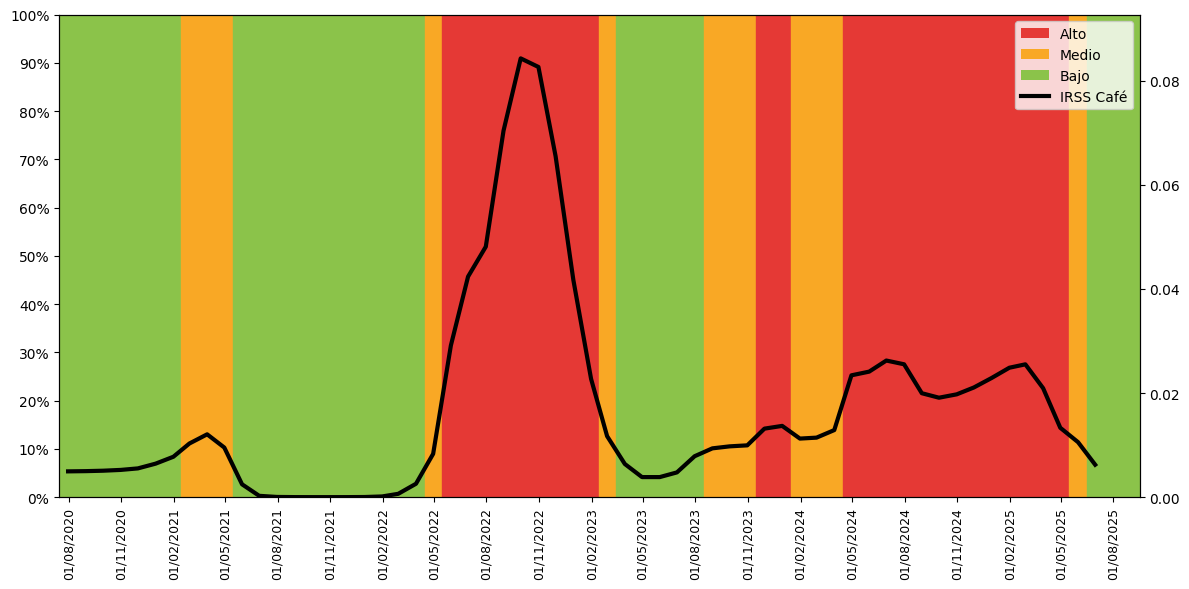
\includegraphics[scale=0.8]{fig3.png}
   \end{center}
      
   La serie mensual del IRSS muestra tres fases claras: 
   
   \begin{itemize}
   \item \textbf{Estrés agudo en 2022:} la cosecha 2022 se vio fuertemente afectada por los daños de la roya, combinados con la caída de los precios internacionales, altos costos logísticos y problemas climáticos y eso provoco disminución de las exportaciones del grano en comparación con ciclos anteriores. 
   
   \item \textbf{Normalización 2023:} A lo largo del 2023, el IRSS mostró un descenso sostenido desde niveles altos hacia el rango de \textbf{Riesgo Medio/Bajo}, reflejando la \textbf{corrección progresiva de los desequilibrios que marcaron el año anterior}. El impacto de los altos costos logísticos y de fertilizantes comenzo a \textbf{moderarse} conforme se normalizaron las rutas marítimas y bajaron los precios internacionales del petroleo, lo que redujo el costo promedio de producción por quintal. 
   \item \textbf{Reputente 2024:} Durante 2024, el IRSS registró un repunte hacia el rango de Riesgo Alto, impulsado por una nueva fase e encarecimiento de costos y deterioro del entorno externo. En el ámbito internacional, el aumento de las tarifas del transporte marítimo y la persistencia de precios elevados del petróleo y sus derivados incrementaron nuevamente los costos logísticos y de fertilizante, presionando los márgenes de rentabilidad del productor. 
   \item \textbf{Mejora 2025:} Durante el primer semestre de 2025, el IRSS mostró una \textbf{tendencia descendente sostenida}, consolidando la \textbf{convergencia del sector al rango de Riesgo Bajo}. Este comportamiento responde a una combinación del factores favorables tanto externos como internos. En el plano internacional, los precios del café arábica se mantuvieron por encima del promedio histórico, impulsados por menores inventarios globales y una demanda estable en los principales mercados compradores. Asimismo, la normalización parcial de los costos logísticos y energéticos tras la desaceleración del WTI y la estabilización de las tarifas marítimas, redujo los costos operativos de los productores, mejorando sus márgenes de rentabilidad. 
   \end{itemize}
En síntesis, la evolución del IRSS entre 2022 y 2025 evidencia la \textbf{capacidad de recuperación del sector cafetalero hondureño} frente a choques externos y condiciones climáticas adversas. La convergencia del índice hacia un nivel de \textbf{riesgo bajo (33.3)} confirma que el sector atraviesa una etapa de \textbf{estabilidad relativa}, aunque persisten \textbf{vulnerabilidades asociadas a la volatilidad de precios internacionales y costos de insumos}. Este desempeño refuerza la importancia de mantener una \textbf{gestión prudencial del crédito agrícola}, con un monitoreo permanente del IRSS y de los factores macroeconómicos que inciden en su comportamiento. 
  \end{block}

\end{column}

\separatorcolumn

\begin{column}{\colwidth}
%====================================================
%                                                        BLOQUE 7
%====================================================
  \begin{exampleblock}{Implicaciones para gestión y crédito}
  
  Desde la óptica de gestión integral de riesgos, se identifican las siguientes implicaciones y líneas de acción: 
  \begin{enumerate}
  \item \textbf{Originación y crecimiento selectivo} \\
  Continuar con una \textbf{política de crecimiento prudencial}, priorizando clientes con historial de pago sólido, prácticas agronómicas verificadas y accesos a mercados diferenciados. Se recomienda diversificar la exposición geográfica, evitando concentración en zonas con alta sensibilidad climática o dependencia de un solo comprador ancla. 
  \item \textbf{Estructura y condiciones de crédito}\\ 
  Mantener esquemas de ago alineados al ciclo productivo del café, con amortizaciones principales posteriores a la cosecha. En escenarios de estrés del IRSS, se sugiere la aplicación táctica de períodos de gracia parciales o reestructurales ligeras, de forma preventiva y bajo análisis caso a caso. 
  \item \textbf{Evaluación y monitoreo:} Incorporar el IRSS como variable de referencia dentro de los comités de crédito y seguimiento de portafolio, activando alertas cuando el índice supere los 40 puntos (riesgo medio) o presente deterioro sostenido durante tres meses consecutivos. Esto permitirá una respuesta temprana ante cambios en las condiciones macro o de mercado. 
  \item \textbf{Sostenibilidad y diferenciación}\\
  Incentivar el financiamiento a \textbf{productores certificado (RFA, Orgánico, FLO)} y con trazabilidad ambiental y social, dado que estos segmentos muestran mayor resilencia ante volatilidad de precios y contribuye también a la alineación con objetivos de sostenibilidad institucional.  
  \item \textbf{Provisión y apetito de riesgo}\\
  Mantener provisiones consistentes con un escenario de \textbf{riesgo bajo}, sin relajar los estándares de evaluación crediticia. En caso de deterioro del IRSS hacia riesgo medio o alto, el portafolio deberá ser revisado y ajustado en límites de exposición y niveles de provisión. 
  \end{enumerate}
El actual posicionamiento del sector café permite sostener un perfil de riesgo estable y manejable, siempre que se mantenga la disciplina en la originación, la diversificación geográfica y el uso del IRSS como instrumento de gestión preventiva. Esta práctica asegura que la estrategia de financiamiento agrícola continúe alineada con los objetivos de rentabilidad ajustada por riesgos definidos  por la organización. 
  \end{exampleblock}
%====================================================
%                                                        BLOQUE 8
%====================================================
  \begin{block}{Perspectivas y próximos paso}
  
  De cara a este segundo semestre del 2025, el sector cafetalero hondureño se mantiene en una posición sólida, respaldada por precios internacionales estables, una oferta global contenida y condiciones climáticas moderadoras. \\[0.4cm]
  
  El modelo IRSS proyecta que, bajo un escenario base de estabilidad de precios y costos, el índice se mantendría en entorno a 34 puntos (riesgo bajo), reflejando la continuidad de un entorno de riesgo acotado y una adecuada capacidad de pago del productor. \\[0.4cm]
  
  No obstante, persisten riesgos latentes que podrían modificar esta tendencia: 
  \begin{itemize}
  \item Un eventual \textbf{descenso en los precios internacionales del café} ante mayor oferta de países competidores (Brasil, Colombia). 
  \item \textbf{Rebotes en los costos energéticos o logísticos}, derivados e tensiones geopolíticas o disrupciones de transporte global. 
  \item \textbf{Anomalías climáticas} asociadas a eventos como huracanes o lluvias excesivas que afecten la calidad y el volumen de la cosecha 2025 - 2026. 
  \end{itemize}
\textbf{Líneas estratégicas de seguimiento para Ficohsa:}\\
\begin{itemize}
\item Incorporar el IRSS en los \textbf{reportes trimestrales de riesgo sectorial} y en el tablero de apetito de riesgo agrícola. 
\item Mantener \textbf{coordinación técnica con IHCAFE} para compartir proyecciones de cosecha, precios y condiciones climáticas. 
\item Reforzar la capacitación del equipo de créditos en herramientas de análisis sectorial y monitoreo de indicadores como el IRSS. 
\end{itemize}

El sector café muestra una recuperación consolidada y un nivel de riesgo bajo, lo que permite mantener la exposición actual dentro de los parámetros prudenciales de Ficohsa. \\[0.4cm]
La aplicación continua del modelo IRSS fortalecerá la capacidad institucional para anticipar riesgos emergentes, alinear decisiones de crédito al apetito definido, y consolidar una visión prospectiva y sostenible del financiamiento agrícola dentro del Grupo Financiero Ficohsa. 
  \end{block}

\end{column}

\separatorcolumn
\end{columns}
\end{frame}

\end{document}
